\section{Data and Preprocessing}
\label{sec:data}

\subsection{Dataset and sentiment mapping}

We use the filtered version of GoEmotions \cite{demszky2020goemotions}: 54,263 comments
(43,410 train, 5,426 dev and 5,427 test), with one or more of 28 labels each. The three files
are joined and every emotion is mapped to positive, negative or ambiguous with the official
\texttt{sentiment\_mapping.json}; neutral is treated as a group of its own. A comment receives
a sentiment only if all its labels fall in the same group; otherwise it is \emph{mixed} (this
includes neutral together with any emotion, 1,751 comments). This rule reproduces exactly the
expected counts: 19,020 positive, 10,217 negative, 4,805 ambiguous, 16,021 neutral and 4,200
mixed (Fig.~\ref{fig:groups}). Only positive and negative comments are kept. The data has no
missing values, no empty texts and no repeated ids.

\begin{figure}[t]
\centering
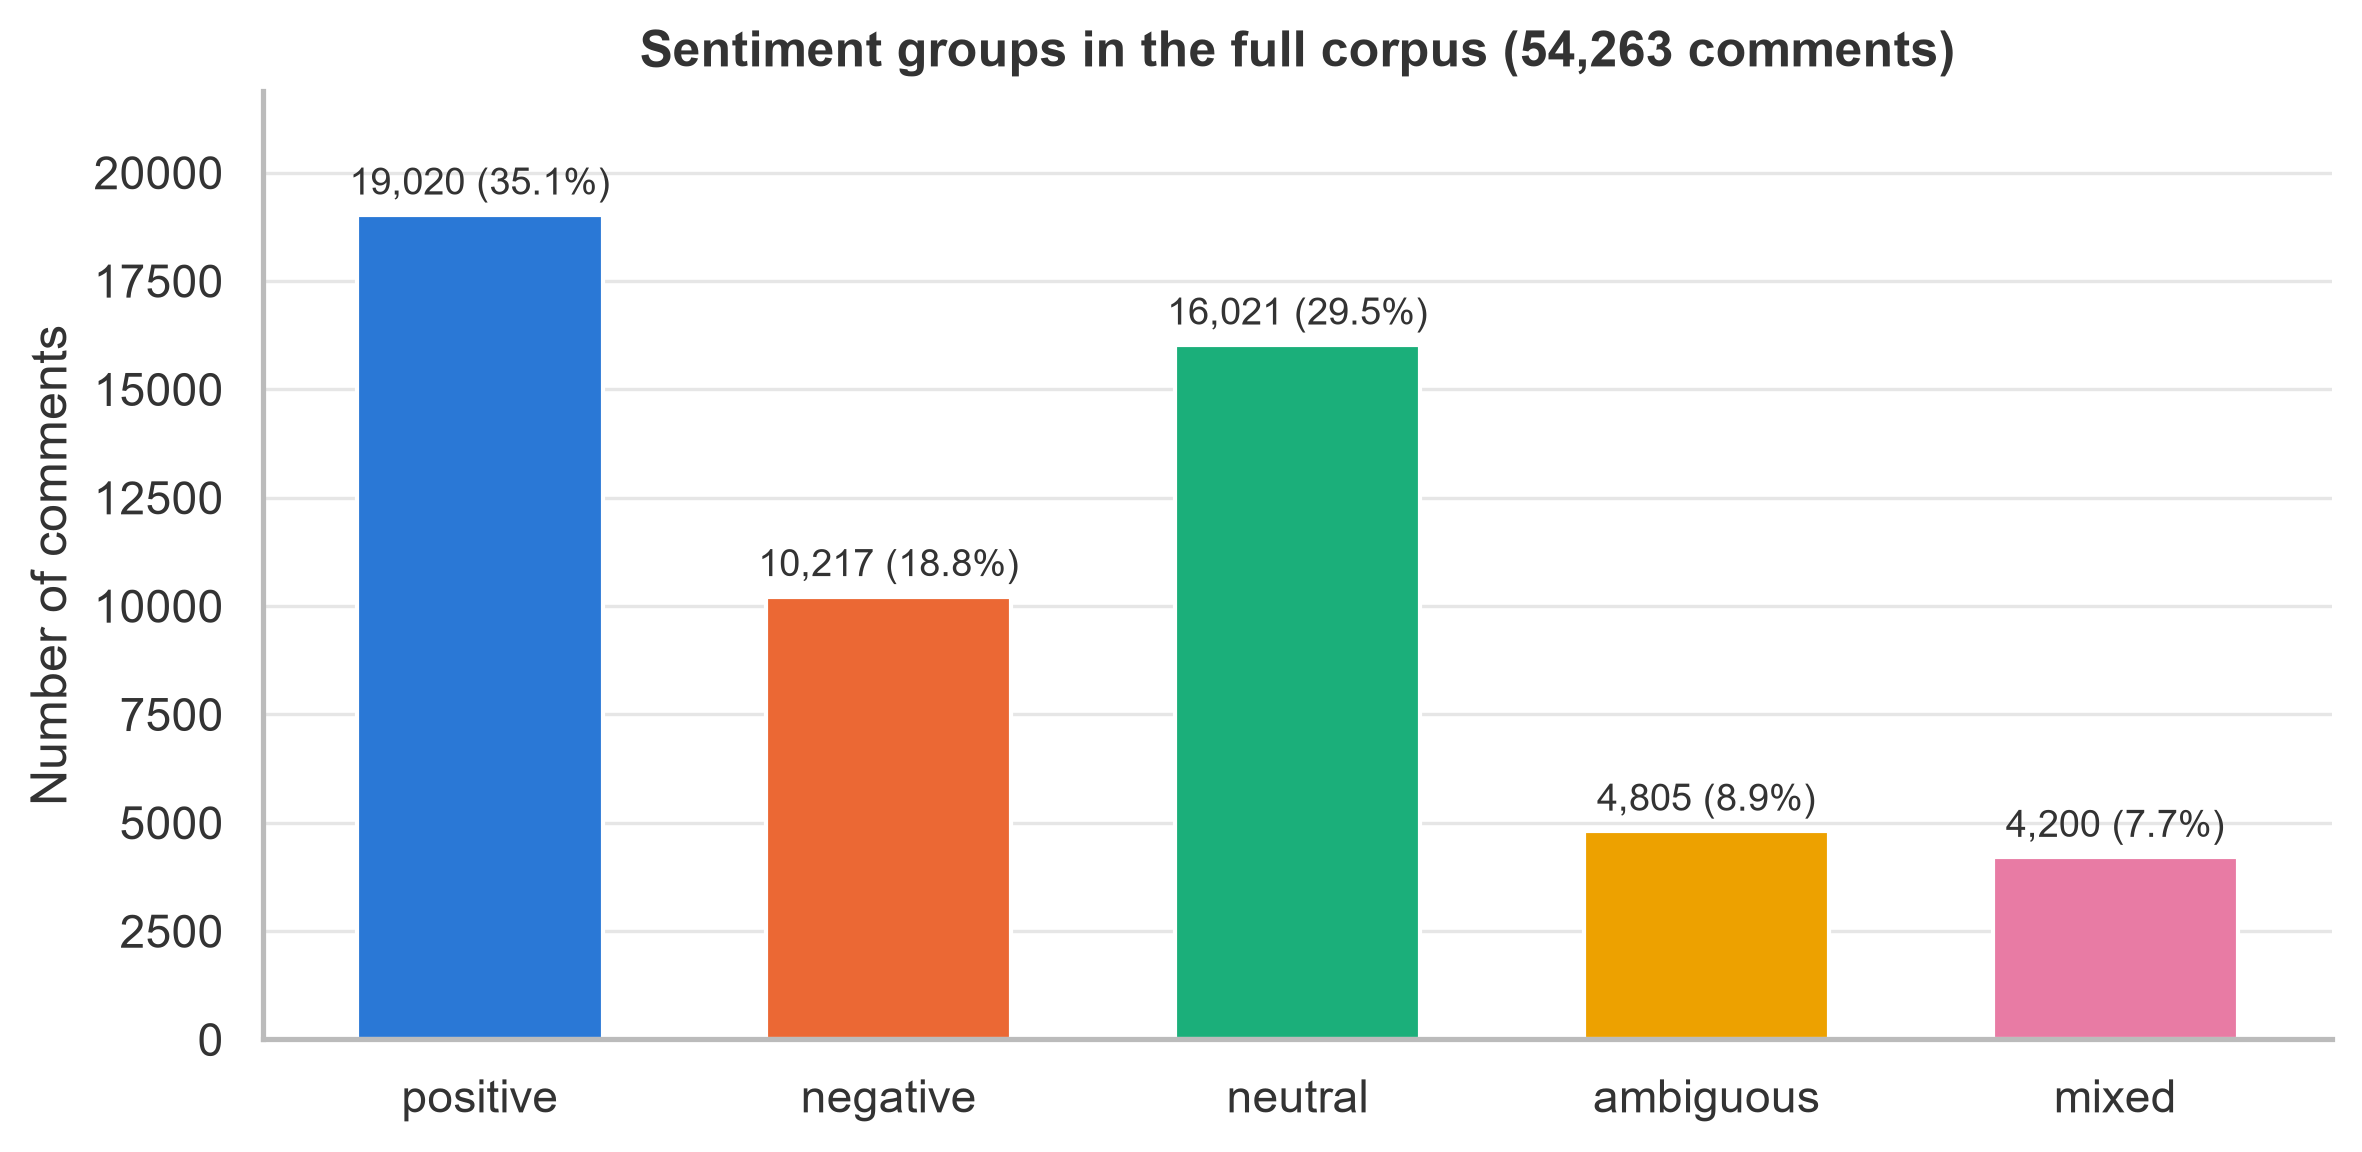
\includegraphics[width=\columnwidth]{eda_sentiment_groups.png}
\caption{Sentiment groups in the 54,263 comments after applying the official mapping.
Positive comments are 1.9 times more frequent than negative ones.}
\label{fig:groups}
\end{figure}

\subsection{Deduplication, balancing and split}

Duplicates are removed before sampling, comparing texts after stripping and lowercasing. Among
the 29,237 positive/negative candidates, 213 exact copies are dropped (mostly short replies such
as ``thank you!''), and one text that appears with both labels (``Weird flex but ok'') is
removed with all its 3 copies, leaving 29,021 comments. From them, 500 positive and 500
negative comments are sampled with \texttt{SEED = 42}, so that the majority baseline is exactly
50\% accuracy. The 1,000 comments are split 80/20 with stratification into 800 training
(400/400) and 200 test comments (100/100), with no text shared between both sets. For
hyperparameter selection, 15\% of the training set (120 comments, stratified) is held out as
validation; the test set is never used to choose a model.

\subsection{Text cleaning}

Each comment is normalized as follows: apostrophes are unified, the placeholders
\texttt{[NAME]} and \texttt{[RELIGION]} become the tokens \texttt{nametoken} and
\texttt{religiontoken}, URLs are removed, emojis are converted to word tokens with
\texttt{emoji.demojize} (e.g.\ \texttt{smiling\_face\_with\_heart\_eyes}), text is lowercased,
negative contractions are expanded (``don't'' $\rightarrow$ ``do not''), and punctuation and
digit-only tokens are removed. Finally the NLTK English stopwords \cite{bird2009natural} are removed
\emph{except negations}: 177 stopwords are dropped while negation words such as \texttt{not},
\texttt{no}, \texttt{nor} and \texttt{never} are kept. Removing negations would turn ``not happy'' into
``happy''. In the balanced set, \texttt{not} appears in 32.6\% of the negative comments and in
16.8\% of the positive ones, and it is the most frequent token of both classes
(Fig.~\ref{fig:unigrams}); with the full stopword list only 3.8\% and 1.8\% of the comments
would keep any negation word. Emojis are rare (25 comments of the balanced set) but are kept
because they carry sentiment.

After cleaning, comments have 6.98 tokens on average (13.05 words before cleaning), the 95th
percentile is 13 and the longest has 20 tokens. We therefore use sequences of length
\texttt{MAX\_LEN = 30}, which truncates no comment; 76.8\% of the positions of the training
matrix are padding.

\begin{figure}[t]
\centering
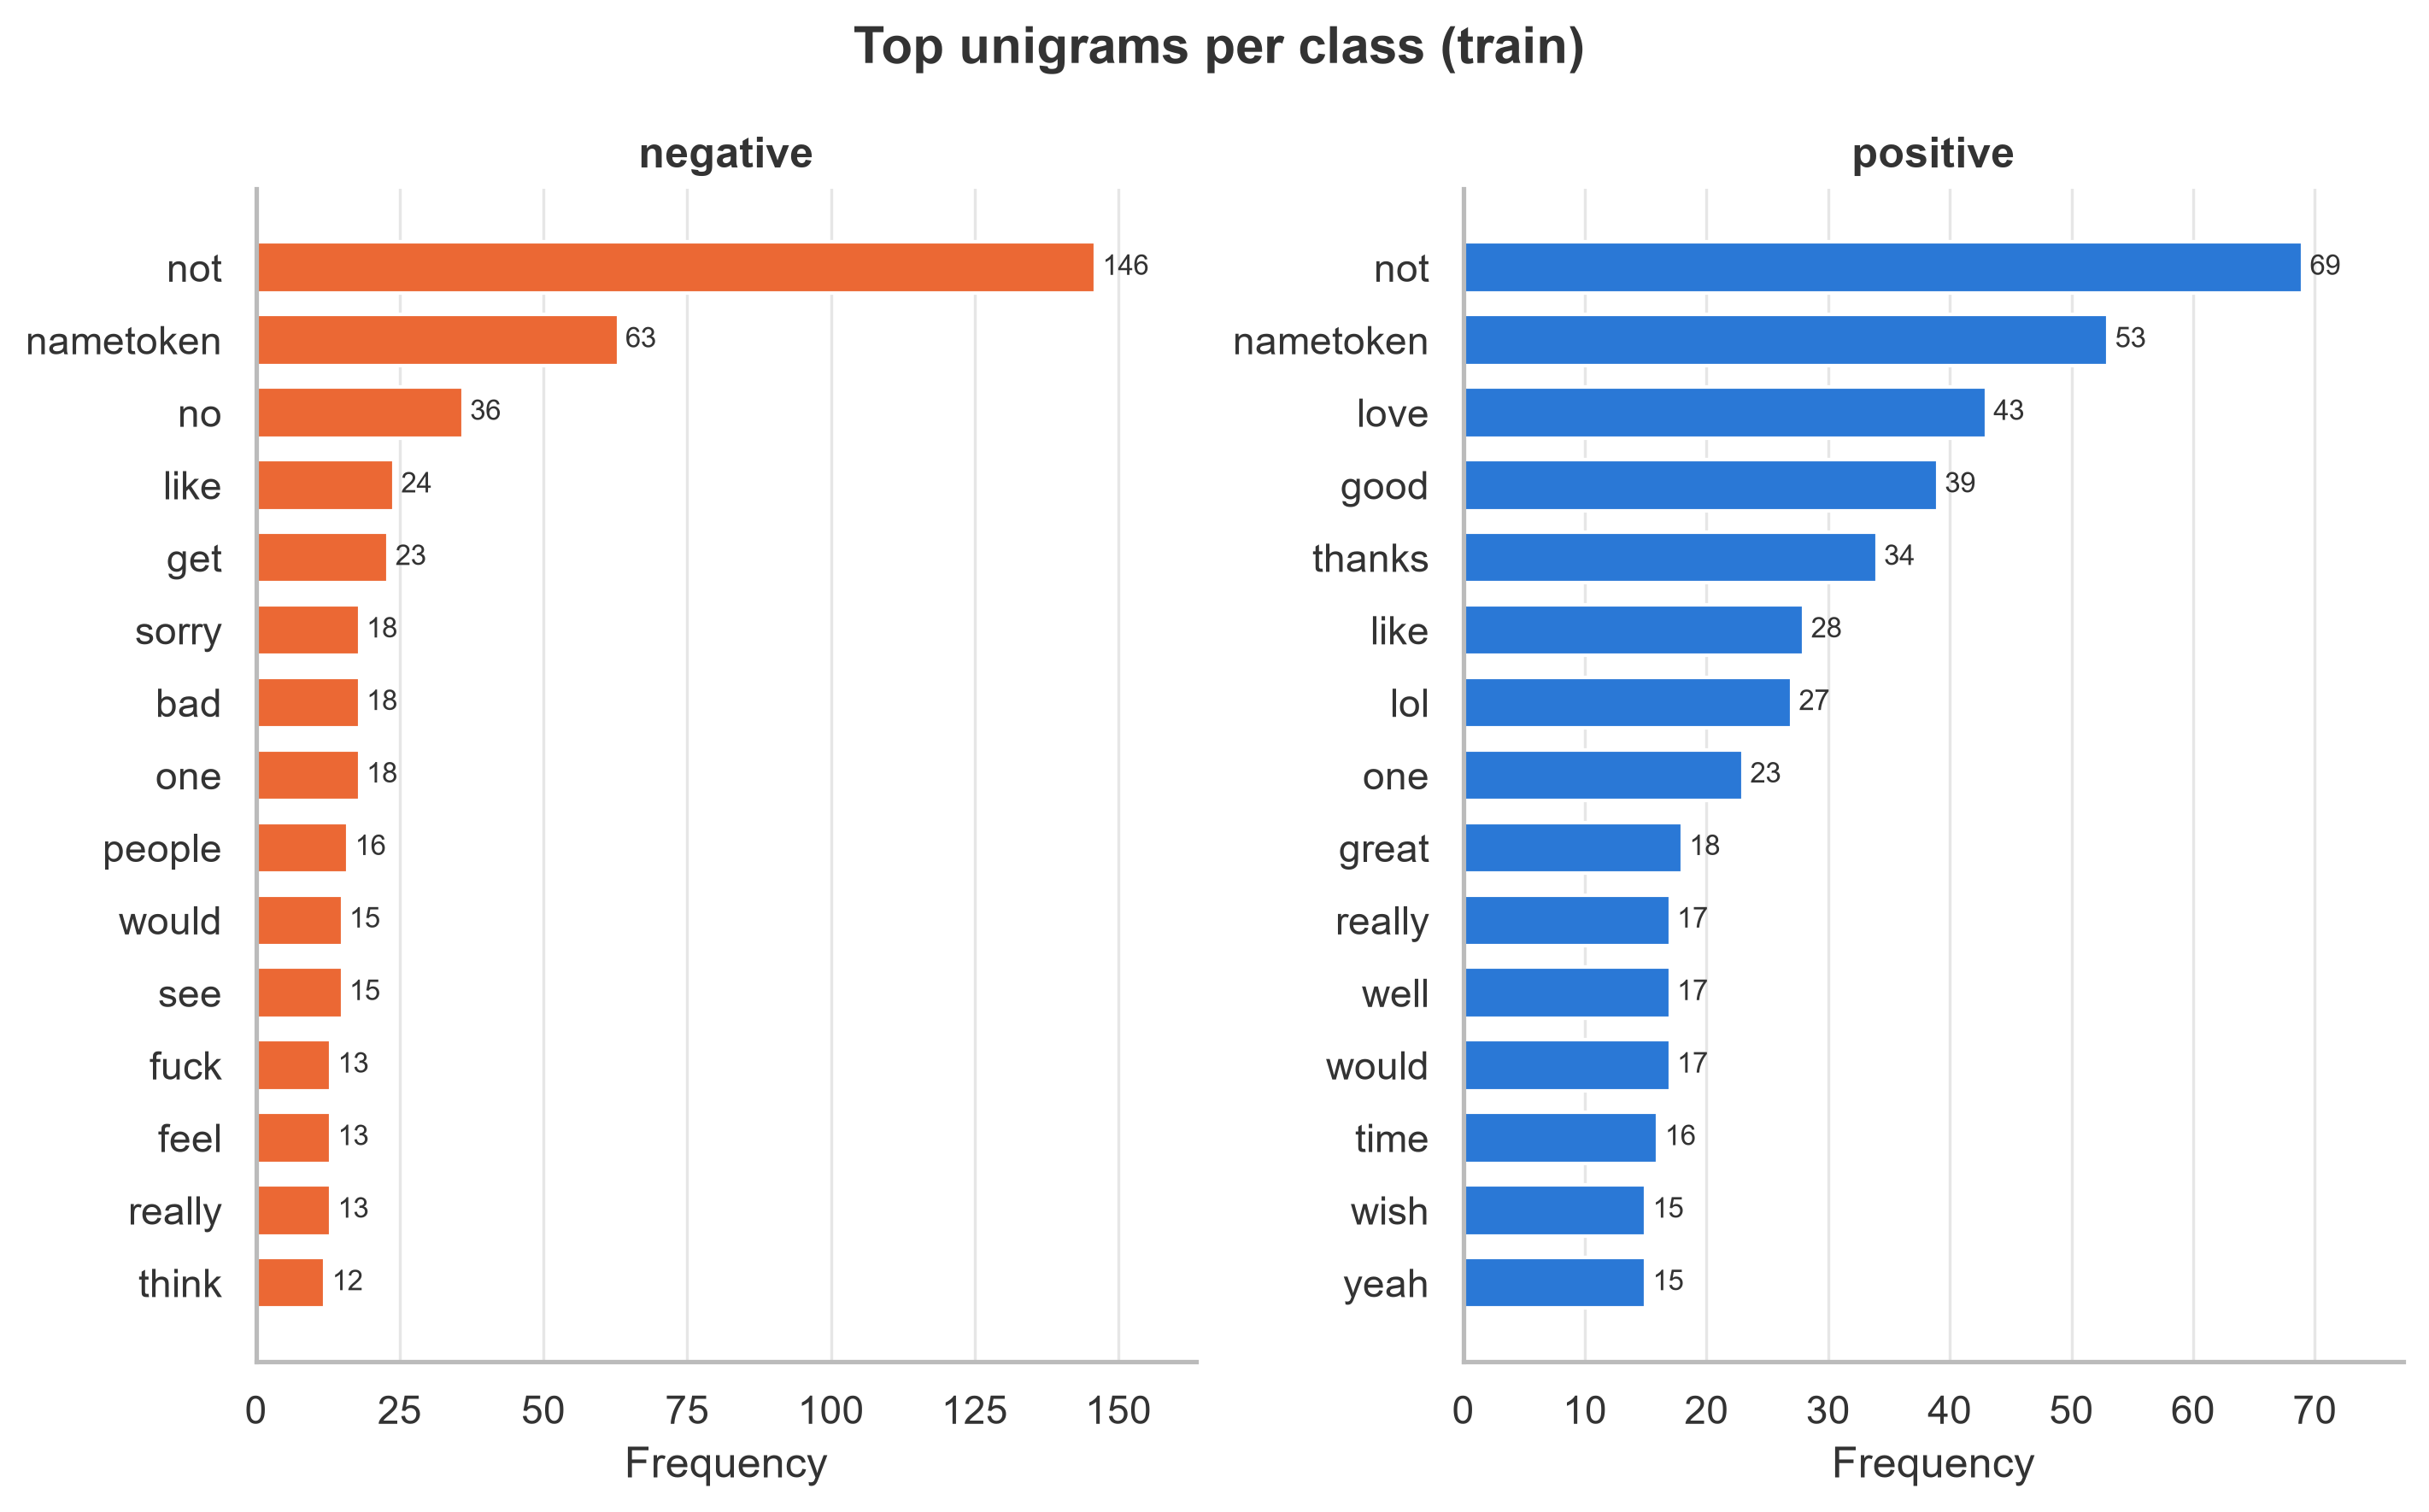
\includegraphics[width=\columnwidth]{eda_top_unigrams.png}
\caption{Most frequent tokens per class in the training set after cleaning. The negation
\texttt{not} is kept and is twice as frequent in negative comments.}
\label{fig:unigrams}
\end{figure}

\subsection{Vectorization}

The Dense, RNN and LSTM models share the same input: a Keras \texttt{TextVectorization}
layer that splits the cleaned text on whitespace and maps every token to an integer, padded to
30 positions. The layer is adapted \emph{only on the training texts}, so no information
from the test set leaks into the features. The vocabulary has 2,364 tokens (2,366 ids with
padding and the unknown token), and 67.6\% of them appear only once. As a consequence, 30.7\% of
the test tokens are out of vocabulary and 162 of the 200 test comments contain at least one
unknown word; the validation split shows a similar rate (28.2\%), so it is a realistic proxy
for the test condition. This sparsity is expected with 800 short comments and is one of the
motivations for the pre-trained Transformer of Section~\ref{sec:transformer}, which uses its
own subword tokenizer on the raw text.
